\documentclass[../main.tex]{subfiles}
\begin{document}
\setchapterstyle{kao}
\setchapterpreamble[u]{\margintoc}
\chapter[Differential forms II]{Differential forms II\footnotemark[0]}
\labch{diff_form_II}
\section*{Settings}
Our starting point will be a differentiable manifold $\mathbf{M}$, at some point we will have some local charts $A=\{(u_{\alpha},\varphi_{\alpha})\}_{\alpha\in A}$. What is relevant for us is that our manifold has a tangent space for every point, so we can assign a 1-form, or more generally a k-form, on each of these linear spaces. If we do it in a smooth way, we will have a differential form. 
\begin{figure}[H]
	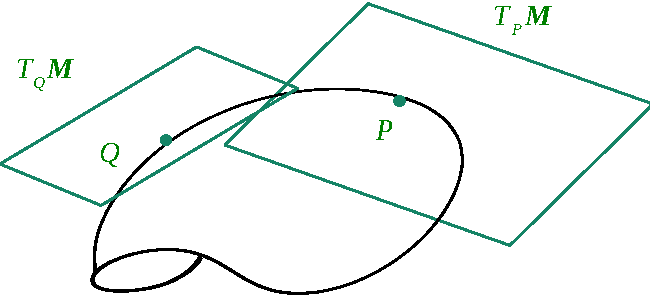
\includegraphics{images/differential_forms_scheme_II.pdf}
	\caption{Scheme of the tangent spaces in the points $P,M\in\mathbf{M}$.}
	\labfig{diff-forms-scheme-II}
\end{figure}
The prototype is the definition of vector field:\marginnote[5mm]{This definition would have been more appropriate in \refch{tang_space}.}
\begin{definition}[Vector field]\index{Vector field}
A vector field is a map
\[\mathbf{M}\ni {\color{red}p}\mapsto v\in T_{\color{red}p} \mathbf{M} \ \textrm{ s. t. the correspondence is smooth}\]
i.e. such that for \textbf{\underline{some}} [and, hence, for \textbf{any}] local chart $(u,\varphi)$ the local decomposition on the coordinate basis $V=\sum_{j=1}^n v^j(p)(e_j)_p$\marginnote{Also the local basis depends on the point, if you change the point the basis changes. We will not be pedantic on this notation, although \cite{doCarmo1994} uses the pedantic one $(e_j)_p$.} provides $\mathbf{C^{\infty}}$\textbf{-smooth functions} $\mathbf{M}\ni p\mapsto v^j(p)\in\mathbb{R}$.
\end{definition}
% 1:30:04
The trick is that we want to define a vector field as an assignment of a vector in every tangent space which is smooth. But we are not allowed to say that is smooth by using the ambient space\sidenote{Because there is no ambient space} and so the trick is to specify that in some chart the components will be smooth. If we change our chart, the components will change, but the smoothness will be preserved, because the change of coordinates is a smooth diffeomorphism and smoothness goes into smoothness. Therefore we have to check it just in one chart to be automatically true in every other chart. Differential 1-forms are similar to a vector field, but instead they use a covector, so they could be referred as covector fields:
\begin{definition}[(Differential) 1-form]\index{Differential 1-form}
A differential 1-form is a map $\alpha$
\[
\mathbf{M}\ni{\color{red}p}\mapsto \alpha_{\color{red}p}\in\Lambda^1 T_{\color{red}p}\mathbf{M}=T_{\color{red}p}^*\mathbf{M}\]
such that for some (and, hence, for any) local chart $(u,\varphi)$ the components with respect to the \textbf{dual basis}\marginnote{The dual basis depends, of course, on the chart.} $\{dx^1,\dots,dx^n\}$ are smooth, i.e. $\alpha=\sum_{j=1}^n\alpha_j(p)(dx^j)_p$ provides $\mathbf{C^{\infty}}$\textbf{-smooth functions} $\mathbf{M}\ni p \mapsto \alpha_j(p)\in\mathbb{R}$.
\end{definition}

\begin{definition}[Differential k-form]\index{Differential k-form}
A differential k-form is a map $\omega$\marginnote{In \cite{doCarmo1994} there is a $\ast$ ($T_P^\ast$), but it should be a typo.} \[\mathbf{M}\ni p\mapsto\omega\in\Lambda^k T_p\mathbf{M}\] such that for some (and, hence, for any) local chart, the components are $\mathbf{C^{\infty}}$\textbf{-smooth}.
\end{definition}

\section{Wedge product of a differential form}
We inherit everything from the linear theory in $E\cong\mathbb{R}^n$. In the following, we will denote with $\Omega^k(\mathbf{M})$ the space of k-differential forms, which is a \textbf{linear space}.

\begin{definition}[Wedge product of a differential form]\index{Wedge product of a differential form}
Let $\omega\in\Omega^k(\mathbf{M})$ and $\eta\in\Omega^l(\mathbf{M})$.
\[
(\omega\wedge\eta)_{\color{red}p}:=\omega_{\color{red}p}\underset{\mathclap{\tikz \node {$\uparrow$} node [below=1ex] {\footnotesize Wedge product in $T_p\mathbf{M}\cong\mathbf{R}^n$ };}}\wedge\eta_{\color{red}p}
\]
\end{definition}

\underline{Rem:} One always has to check that $p\mapsto(\omega\wedge\eta)_p$ is still $\mathbf{C}^{\infty}$\textbf{-smooth}. You can do it in a local chart .

\section[Exterior derivative (Cartan)]{Exterior derivative\sidenote{"\href{https://it.wikipedia.org/wiki/Derivata_esterna}{Derivata esterna}" in Italian.} (\href{https://it.wikipedia.org/wiki/\%C3\%89lie_Joseph_Cartan}{Cartan})}\begin{marginfigure}
	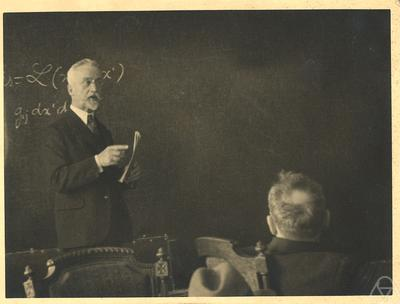
\includegraphics[width=1\linewidth]{images/ElieCartanMFO.jpg}
	\caption[Élie Cartan's photo]{From \href{https://commons.wikimedia.org/wiki/File:ElieCartanMFO.jpg}{Wikimedia}: Élie Cartan's photo, album linked to the Mathematical Seminar in Hamburg (Germany). Élie Joseph Cartan (French; 9 April 1869 – 6 May 1951) was an influential French mathematician who did fundamental work in the theory of Lie groups, differential systems (coordinate-free geometric formulation of PDEs), and differential geometry. He also made significant contributions to general relativity and indirectly to quantum mechanics. He is widely regarded as one of the greatest mathematicians of the twentieth century.}
	\labfig{ElieCartan}
\end{marginfigure}
For convenience, we define the 0-forms as (smooth) functions, so the space $\Omega^0(\mathbf{M})$ corresponds to $\mathbf{C}^{\infty}(\mathbf{M})$. The idea of Cartan was to build an universal differential, which is intrinsic, i.e. it does not depend on the local coordinates:

\[
\Omega^0(\mathbf{M})\xrightarrow[]{\textrm{d}}\Omega^1(\mathbf{M})\xrightarrow[]{\textrm{\textrm{d}}}\Omega^2(\mathbf{M})\xrightarrow[]{\textrm{d}}\Omega^3(\mathbf{M})
\]

$\textrm{d}$ must be compatible with the \textbf{linear structure}, with the \textbf{wedge product}\sidenote{We would like to have it Leibniz, but actually it is impossible. It is Leibniz up to a sign.} and with the fact that:

\[
\begin{split}
\Omega^0(\mathbf{M}) & \xrightarrow[]{\textrm{d}} \Omega^1(\mathbf{M})\\
f &\mapsto \textrm{d}f
\end{split}
\]

$\textrm{d}f$ should be the usual differential of a function $f:\mathbf{M}\xrightarrow[]{\mathbf{C}^{\infty}}\mathbb{R}$ (\refch{tang_space}), i.e.
\[
\textrm{d}f_p: T_p\mathbf{M}\xrightarrow[]{}\mathbb{R} \ \textrm{with} \ \textrm{d}f_p\in T_p^*\mathbf{M} \quad  \text{\parbox{3 cm}{\centering linear 1-form \\[-4pt]  at every point}}
\]
defined as:
\[
\textrm{d}f_p([\gamma])=\frac{\textrm{d}}{\textrm{d}t}(f\circ\gamma)(t)\big|_{t=0}\overset{\textrm{L.C.}}{=}\sum_j\frac{\partial f}{\partial x^j}\left(x(\gamma(0))\right)v^j
\]


\begin{theorem}[E. Cartan]
There exists a unique\footnote{And therefore it is an intrinsic object.} map $\dd:\Omega^k(\mathbf{M})\xrightarrow[]{}\Omega^{k+1}(\mathbf{M})$ such that:
\begin{enumerate}
    \item $\dd$ is \textbf{linear}
    \item $\dd$ is \textbf{pseudo-Leibniz}: $\dd(\omega\wedge\eta)=\dd\omega\wedge\eta{\color{red}+(-1)^{\text{\textrm{deg}}\omega}}\omega\wedge d\eta\\ \forall\omega\in\Omega^k(\mathbf{M}),\eta\in\Omega^l(\mathbf{M})$
    \item if $\phi\in\Omega^0(\mathbf{M})=\mathbf{C^{\infty}(\mathbf{M})}$, then $\dd\phi$ is the ordinary differential (see above);
    \item $\textrm{d}^2=0:\forall\omega\in\Omega^k(\mathbf{M})$ one has $d({\color{red}d\underset{\mathclap{\tikz \node {$\uparrow$} node [below=1ex] {\footnotesize (k+1)-form };}}\omega})=0$.
\end{enumerate}
\end{theorem}
We never introduced one, but in a local chart, if $\omega\in\Omega^k(\mathbf{M})$ has local expression $\omega=\sum\omega_I(x)\textrm{d}x^I$, \marginnote{With $I$ we denote the set $(i_1,\dots,i_k)$ such that $i_1<\dots<i_k$ and with $dx^I$ we denote $dx^{i_1}\wedge\dots\wedge dx^{i_k}$} then $\textrm{d}\omega$ can be written as:
\[
\textrm{d}\omega=\sum(\textrm{d}\omega_I(x))\wedge dx^I \qquad \Big|\Big| \quad \star
\]
\begin{proof}
See \sidecite{von1978differential} omitted here.
\end{proof}
%INIZIO LEZIONE 7 - 24/03/2022
\begin{kaobox}[frametitle=Remark]
The "opposite" approach is also possible. One might define the exterior differential via ($\star$), and then prove that it satisfies properties (1)-(4) and it is \textbf{intrinsic} (i.e. independent of the choice of a chart).
\end{kaobox}
\begin{kaobox}[frametitle=Remark]
There exists also the \textbf{Lie derivative} of a differential form $\omega\in\Omega^k(\mathbf{M})$ along a vector field $V\in\nu(\mathbf{M})$ denoted by:
\[
\mathcal{L}_V\omega
\]
This topic will not be covered here\footnote{But it is covered in Capitolo 8 of \cite{ferrari2020general}.}.
\end{kaobox}
\subsection{Examples}
For a physicist, what is important is to learn how to use the exterior differential, so we now see some examples.\\
\paragraph{\underline{$k=0$}}Let $\phi\in \Omega^0(\mathbf{M})=C^\infty(\mathbf{M})$:
\[
\textrm{d}\phi(V) \overset{\textrm{L.C.}}{=}\sum\frac{\partial\phi}{\partial x^j}(x)v^j
\]
Since $v^j=dx^j(V)$, one can also write:
\[
\textrm{d}\phi=\sum_j\frac{\partial\phi}{\partial x^j}(x)dx^j
\]
Let us notice that it has the same information of the gradient, but with a little important difference: the differential applied to $V$ is intrinsic. If you want to write it as a matrix, it should be written like:
\[
\textrm{d}\phi(V)=\underbrace{\left(\frac{\partial \phi}{\partial x^1}, \dots, \frac{\partial \phi}{\partial x^n}\right)}_{\textrm{covariant}}
\overbrace{
\begin{pmatrix}
v^1\\
\vdots\\
v^n
\end{pmatrix}
}^{\textrm{contravariant}}
\]
If we change local chart, both of them will change according to the Jacobian matrix of the transformation, but they will change the opposite way and the two Jacobian matrices will cancel each other $JJ^{-1}$, leaving the same intrinsic object. Contrast to the \textbf{gradient}\index{Gradient}, which is a vector, whose j component is the j-derivative.\sidenote{If we use the Ricci's rule we see immediately that something is wrong with the index, this is because we need to put a metric.} 
\[
\left(\grad \phi\right)^j(x)=\sum_l\delta^{ij}\frac{\partial\phi}{\partial x^l}(x)
\]
The information they contain is the same, but the first is much more natural when we change coordinates.
\paragraph{\underline{$k=1$}} Suppose we have a one form:
\[
\alpha \in \Omega^1(\mathbf{M}) \qquad \alpha = \sum_j A_j(x)dx^j
\]
Let us differentiate $\alpha$:
\[
\begin{split}
\textrm{d}\alpha
&=\sum_j\left({\color{red} \textrm{d}}A_j(x)\right){\color{red}\wedge}dx^j=\\
&=\sum_j\sum_l\frac{\partial A_j}{\partial x^l}(x)dx^l{\color{red}\wedge}dx^j=\\
&=\sum_{\color{red}l<j}\frac{\partial A_j}{\partial x^l}(x)dx^l\wedge dx^j+\sum_{\color{red}l\geq j}\frac{\partial A_j}{\partial x^l}(x)dx^l\wedge dx^j
\end{split}
\]
notice that $dx^l\wedge dx^j=0$ when $l=j$ ($\alpha \wedge\alpha=0$ \textbf{always!}) and moreover that $dx^2\wedge dx^1={\color{red}-}dx^1\wedge dx^2$. So we can reorder the indices in the second sum and obtain:\marginnote{The final formula is without the green comment.}
\[
\textrm{d}\alpha=\sum_{\color{red}l<j}\underbrace{\left(\frac{\partial A_j}{\partial x^j}(x){\color{red}-}\frac{\partial A_l}{\partial x^j}(x)\right)}_{\color{teal} \left(\textrm{rot}\Vec{A}\right)_{lj}}dx^l\wedge dx^j
\]
This is something failiar, identifying $\alpha$ with a vector field (neglecting that the indices are downstairs).
\[
\alpha = \sum_j A_jdx^j \ \longleftrightarrow \ \Vec{A}=\left(A_1,A_2,A_3\right)
\]
\paragraph{\underline{$k=2$}} Suppose to have:
\[
\eta \in \Omega^2(\mathbf{M}) \quad \eta = \sum_{i<j} \eta_{ij}(x)dx^i\wedge dx^j
\]
We can differentiate by applying the rule:
\[
\begin{split}
\textrm{d}\eta
&=\sum_{i<j}\left({\color{red} \textrm{d}}\eta_{ij}(x)\right){\color{red}\wedge}dx^i\wedge dx^j=\\
&=\sum_{i<j}\sum_l\frac{\partial \eta_{ij}(x)}{\partial x^j}dx^l{\color{red}\wedge}dx^i\wedge dx^j=\\
&=\textrm{reorder}=\\
&=\sum_{l<i<j}\Big(\quad\Big)dx^l\wedge dx^i\wedge dx^j
\end{split}
\]
Explicitly, for the case in which the dimension of the manifold is $n=\textrm{dim}\mathbf{M}=3$ one has:\marginnote{It is usual to take a different basis. We want to identify them with the canonical basis, but this works only in $\mathbb{R}^3$}
\[
\eta=P(x)\underbrace{dx^2\wedge dx^3}_{\color{teal} e_1}+Q(x)\underbrace{dx^3\wedge dx^1}_{\color{teal} e_3\wedge e_1 = e_2}+R(x)\underbrace{dx^1\wedge dx^2}_{\color{teal} e_1\wedge e_2 = e_3}
\]
Then we take, according to our rule:
\[
\textrm{d}\eta=\left(\sum_j \frac{\partial P}{\partial x^j}\textrm{d}x^{\color{red}j}\right)\wedge dx^2\wedge dx^3+\left(\sum_l \frac{\partial Q}{\partial x^l}\textrm{d}x^l\right)\wedge dx^3\wedge dx^1+\left(\sum_m \frac{\partial R}{\partial x^m}\textrm{d}x^m\right)\wedge dx^1\wedge dx^2
\]
We notice that the first sum is non-null just for one value of $j$:
\[
\exists ! \ j \ \textrm{such that} \ dx^j\wedge dx^2 \wedge dx^3 \neq 0, \ \textrm{namely} \ {\color{red} j=1}
\]
The same is true for $l$ and $m$:\marginnote{The first term is already in order}
\[
\begin{WithArrows}
\textrm{d}\eta 
&= \frac{\partial P}{\partial x^1}dx^{1}\wedge dx^2\wedge dx^3+ \frac{\partial Q}{\partial x^2}dx^{2}\wedge dx^3\wedge dx^1+ \frac{\partial R}{\partial x^3}dx^{3}\wedge dx^1\wedge dx^2=\Arrow{reordering}\\
&=\underbrace{\left(\frac{\partial P}{\partial x^1}+ \frac{\partial Q}{\partial x^2}+ \frac{\partial R}{\partial x^3}\right)}_{\textrm{Divergence of }\Vec{F}=\left(P,Q,R\right)}dx^1\wedge dx^2\wedge dx^3
\end{WithArrows}
\]
The exterior derivative of differential forms generalize all the differential operators of vector analysis (gradient, curl, divergence).
\section{Comparison with vector analysis}
\[
\text{\parbox{4 cm}{\centering Differential form \\[-4pt]  {(XX century)}}}\simeq\text{\parbox{4 cm}{\color{teal} \centering Vector Analys \\[-4pt]  (XIX century)}}
\]
\begin{figure}[H]
	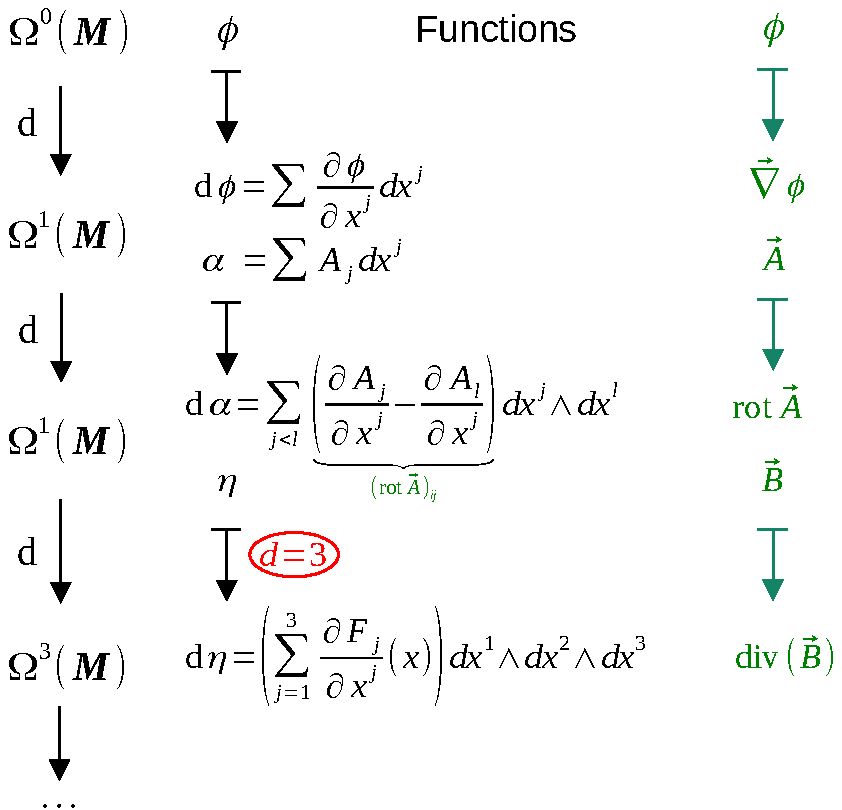
\includegraphics{images/schema_confronto_diff_analisi.pdf}
	\caption[Scheme of the comparison between differential forms and vector analysis]{Scheme of the comparison between differential forms and vector analysis. At some point the chain will stop, because on a manifold of dimension $n$ you can have differential forms up to degree $n$. As we have seen in \vrefch{diff_form_I}, dimension $3$ is somehow "special" since allows us to identify vector fields with 2-forms (instead, given a metric, the identification with 1-forms is always possible).}
	\labfig{schema-confronto-diff-analisi}
\end{figure}
The correspondence between differential forms and vector fields is not so innocent as the schetch in \reffig{schema-confronto-diff-analisi} may let us think. If we want to do it precisely and to write an isomorphism between spaces, we need to introduce a metric and use the so-called \href{https://en.wikipedia.org/wiki/Hodge_star_operator}{Hodge duality}, but since it is not so central for us, we will leave it as a starred exercise.\marginnote[-80mm]{The "\href{https://en.wikipedia.org/wiki/Curl_(mathematics)}{Curl}" should be denoted as "curl", but since the professor is habituated to the Italian notation, he uses "rot", as in \textit{rotore}.}\\
{\fontencoding{U}\fontfamily{futs}\selectfont\char 66\relax} Message: Cartan differential \textbf{d} is a simultaneous generalisation of the operators of vector analysis ($\vec{\nabla}, \textrm{rot}, \textrm{div}, \dots$) and, with respect to that
\begin{enumerate}
    \item The universal property $\textrm{d}^2=0$ generalized
    \begin{enumerate}
        \item \(\ \ \textrm{rot}\ \vec{\nabla}\phi(x)=0 \qquad \textrm{d}\left(\textrm{d}\phi\right)=0\)
        \item \(\textrm{div}\ \textrm{rot}\vec{F}(x)=0 \qquad \textrm{d}\left(\textrm{d}\alpha\right)=0\)
    \end{enumerate}
    \item The \textbf{pseudo-Leibniz property}\index{Pseudo-Leibniz property} generalizes:
    \begin{enumerate}
        \item $\vec{\nabla}\left(\phi\psi\right)=\vec{\nabla}\phi\cdot\psi+\phi\vec{\nabla}\psi$
        \item \(\textrm{rot}\left(\varphi\vec{V}\right)=\vec{\nabla}\varphi\times\vec{V}+\varphi \ \textrm{rot}\vec{V}\)
        \item \(\textrm{div}\left(\varphi\vec{V}\right)=\vec{\nabla}\varphi\cdot\vec{V}+\varphi \ \textrm{div}\vec{V}\)
        \item \(\textrm{div}\left(\vec{X}\wedge\vec{Y}\right)=\textrm{rot}\vec{X}\cdot\vec{Y}\ {\color{red}\underset{\mathclap{\tikz \node {\color{red}$\uparrow$} node [below=1ex] {\footnotesize \color{red} \underline{minus!} };}}{-}}\ \vec{X}\cdot\vec{Y}\)
    \end{enumerate}
    everything with $\textrm{dim}\mathbf{M}=3$
\end{enumerate}
\section{\href{https://it.wikipedia.org/wiki/Henri_Poincar\%C3\%A9}{Poincaré} lemma and its converse}
% \begin{marginfigure}
%     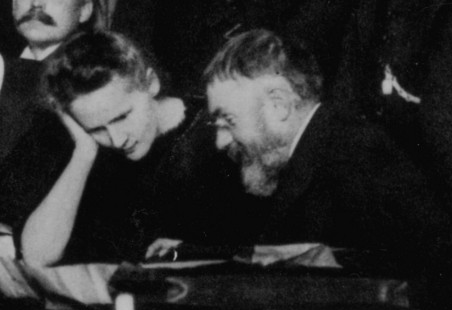
\includegraphics[width=1\linewidth]{images/Curie_and_Poincare_1911_Solvay.jpg}
% 	\caption[Photo of Poincaré and Curie]{From \href{https://commons.wikimedia.org/wiki/File:Curie_and_Poincare_1911_Solvay.jpg}{Wikimedia}: Marie Curie and Poincaré talk at the 1911 Solvay Conference.}
% \end{marginfigure}
\begin{marginfigure}[-20mm]
	\includegraphics[width=1\linewidth]{images/Henri_Poincaré-2.jpg}
	\caption[Photo of Poincaré]{From \href{https://commons.wikimedia.org/wiki/File:Henri_Poincar\%C3\%A9-2.jpg?uselang=it}{Wikimedia}: Jules Henri Poincaré (29 April 1854 – 17 July 1912) was a French mathematician, theoretical physicist, engineer, and philosopher of science. He is often described as a polymath, and in mathematics as "The Last Universalist", since he excelled in all fields of the discipline as it existed during his lifetime.}
	\labfig{Poincaré}
\end{marginfigure}
In vector analysis we use to ask ourselves if a vector field is the gradient of some potential, and we know that this happens if the field is conservative\sidenote{the rotational curl vanishes}and the space is nice\sidenote{It is simply connected, like the full $\mathbb{R}^n$}. The same problems appears with the differential forms: we can ask ourselves if it happens that our differential form is the differential of a lower degree form, i.e. when it happens that a k-form is the Cartan differential of a (k-1)-form.
\begin{kaobox}[frametitle=Terminology]
A k-form $\omega\in\Omega^k(\mathbf{M})$ is \textbf{closed}\index{Closed k-form} if ${\color{red}\textrm{d}\omega=0}$.\\
A k-form $\omega\in\Omega^k(\mathbf{M})$ is \textbf{exact}\index{Exact k-form} if $\exists \ \alpha\in\Omega^{\color{red}k-1}(\mathbf{M})$ such that ${\color{red}\textrm{d}\alpha=\omega}$
\end{kaobox}
There is a result, historically known as Poincaré lemma, that for our viewpoint is trivial because he lived before the time of Cartan.
\begin{lemma}[\href{https://it.wikipedia.org/wiki/Lemma_di_Poincar\%C3\%A9}{Poincaré lemma}]\index{Poincaré lemma}\lablemma{Poincaré}
Any \textbf{exact form is closed.}
\end{lemma}
\begin{proof}
If $\omega$ is exact, then $\omega = \textrm{d}\alpha$ for some $\alpha\in\Omega^{k-1}(\mathbf{M})$. Then $\textrm{d}\omega=\textrm{d}\left(\textrm{d}\alpha\right)=0$.
\end{proof}
What it is not obvious is the converse, that in general is false.\\
\underline{Problem:} Given a \textbf{\underline{closed}} $\omega\in\Omega^k(\mathbf{M})$, it is true that $\exists \ \alpha \in \Omega^{k-1}(\mathbf{M})$ such that $\textrm{d}\alpha=\omega$??\\
\underline{Answer:} In general \underline{\textbf{no!!}} There might be \textbf{topological obstruction} related to "holes" of $\mathbf{M}$.\marginnote[-35mm]{The fact that is closed, it is not sufficient to guarantee that the form is exact. This is the generalization (or the counterpart) of what happens in vector analysis: the fact that a vector field is irrotational, does not always implies that is the gradient of some potential function, because you need the space to be simply connected (a loop must be continuously deformed to zero). The same happens for a divergence free vector field.}

But if you are in some nice manifold, then it works. Hence it does not only depend on the form (vector field), but it depends also and crucially on the structure of the manifold (it will not be the same to be in a sphere or a torus or something else). There are several examples of that:
\begin{marginfigure}[-10mm]
    \centering
	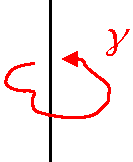
\includegraphics[width=0.5\linewidth]{images/ex1_topol_obstruction.pdf}
	\caption{Example one of topological obstruction}
	\labfig{ex-1-top-obs}
\end{marginfigure}
\begin{marginfigure}
    \centering
	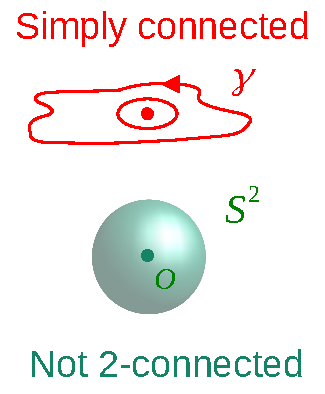
\includegraphics[width=0.6\linewidth]{images/ex2_topol_obstruction.pdf}
	\caption{Example two of topological obstruction.}
	\labfig{ex-2-top-obs}
\end{marginfigure}
\begin{example}
\underline{$k=1$}: If we are interested in 1-forms and we take the real 3D space minus an infinite wire $\mathbf{M}=\mathbb{R}^3\slash \left\{\left(0,0,z\right): z\in\mathbb{R}\right\}$. We see that this is not simply connected. There are some loops which are not continuously deformable to a point \textbf{in} $\mathbf{M}$, therefore \[\exists \ \alpha \in \Omega^1(\mathbf{M})\ \textrm{ one form which is closed but \textbf{not exact}}\]
\end{example}
\begin{example}
\underline{$k=2$}: If we are interested in 2-forms, we take $\mathbf{M}=\mathbb{R}^3\slash \left\{\left(0,0,0\right)\right\}$. In this case every loop can be deformed to the trivial loop (it is simply connected), which is identical to a point, but is not 2-connected: it is not true that every 2-sphere can be continuously deformed to a point. Therefore
\[\exists \ \beta \in \Omega^2(\mathbf{M})\ \textrm{ two form which is closed but \textbf{not exact}}\]
\end{example}
\underline{Details:} Book \cite{von1978differential} or \cite{doCarmo1994}.\\
The way-out from this problem is assuming that our manifold is good enough. Otherwise there could be some interesting effect, for example a magnetic field that does not admit a vector potential is interesting in itself. For some application, it is even more interesting than the ordinary case. Anyway, for very nice space the following proposition holds true.\marginnote{Extra, from Chapter 4 of \cite{doCarmo1994_4}.

\textbf{Definition}. A differential manifold $\mathbf{M}$ is \textit{contractible} (to some point $p_0\in\mathbf{M}$) if there exists a differentiable map $H:\mathbf{M}\times\mathbb{R}\to\mathbf{M},\,H(p,t)\in\mathbf{M},p\in\mathbf{M},t\in\mathbb{R}$ such that
\[
H(p,1)=p,\quad H(p,0)=p_0,\quad \textrm{for all }p\in\mathbf{M}
\]}
\begin{proposition}[Converse to Poincaré lemma]\lablemma{Converse-to-Poincaré-lemma}
Let $\mathbf{M}$ be a manifold. Suppose that $\mathbf{M}$ is \textbf{contractible}\footnote{$\mathbf{M}$ can be \textbf{continuously} deformed to a single point (ex: $\mathbf{M}=\mathbb{R}^d$).}. Then for any $\omega\in\Omega^k(\mathbf{M})$ we have the fact that:
\[
\textrm{d}\omega=0 \ \underset{\mathclap{\tikz \node {$\uparrow$} node [below=1ex] {\footnotesize $\mathbf{M}$ contractible };}}{\Rightarrow} \ \exists \ \eta\in\Omega^{k-1}(\mathbf{M}) \ \textrm{ such that } \ \textrm{d}\eta = \omega
\]
\end{proposition}
This is a general result, if you are interested in 1-form or 2-forms, there are more specific results.
\section[Pull-back of differential forms]{\href{https://it.wikipedia.org/wiki/Pull-back}{Pull-back}\sidenote{"Regressione" in Italian, but also in Italian is used "Pull-back".} of differential forms}
Consider a smooth map and a differential form of degree $k$ on the target (arrival) space as in \reffig{pull-back}:
\[
\mathbf{M}\xrightarrow[f]{C^\infty}\mathbf{N}, \quad \omega \in \Omega^k(\mathbf{N})
\]
\begin{figure}[H]
	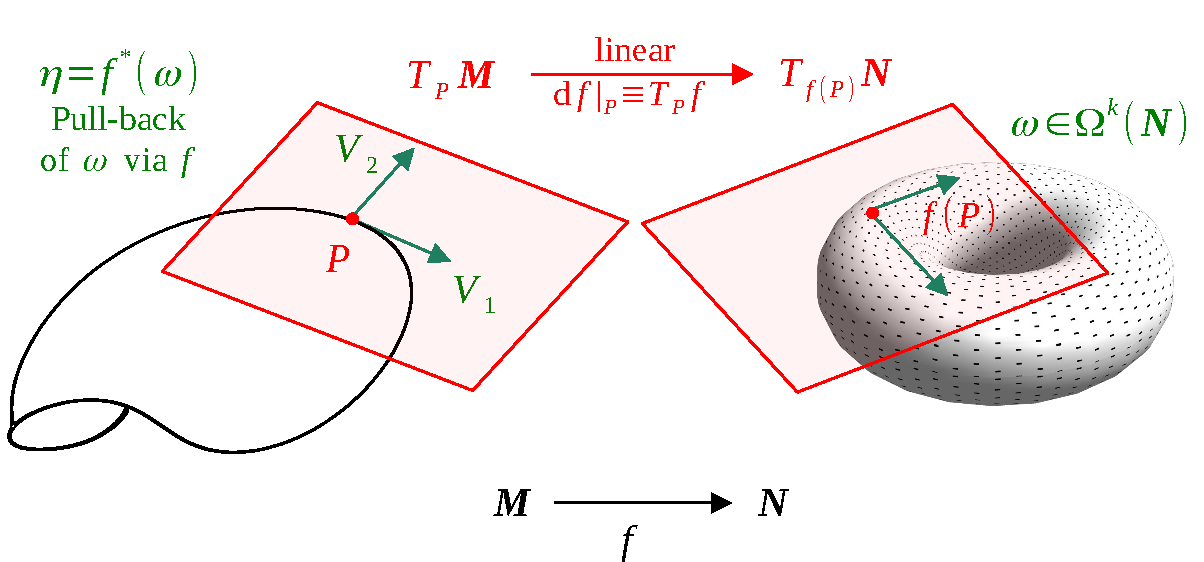
\includegraphics{images/pull_back.pdf}
	\caption{Pull-back of a differential form. The notation of the linear map changes accord to the book.}
	\labfig{pull-back}
\end{figure}
We want to construct a differential form $\eta$ of the same degree on manifold $\mathbf{M}$ of the source space, which will be obtained by $\omega$ by pulling it back.\sidenote{"Tirandola indietro" in Italian. For this reason is called the "Pull-back" of $\omega \textrm{ via } f$.} We want to define the pull-back $f^\ast(\omega)_P$ in a natural way. We want it to produce a number when applied to vectors, and the only thing we have in our hands is $\omega$. Therefore, it should be related to the only natural point $f(P)$ and the corresponding vectors in the tangent space on the arrival space. To relate them we can use the differential of a map, that maps every green vector in two green vectors on the arrival space. Therefore:
\[
{\color{red} f^\ast(\omega)_P}\left(V_1,\dots,V_k\right):= {\color{red}\omega_{f(P)}}\left({\color{red}\textrm{d}f_P}(V_1),\dots,{\color{red}\textrm{d}f_P}(V_K)\right)
\]
$\textrm{with } \ V_1,\dots,V_k \in T_P\mathbf{M}$. This "natural" definition provides a k-form $\eta\in\Omega^k(\mathbf{M})$ which is called the \textbf{pull-back of $\omega$ via $f$}\index{Pull-back of diff. forms}. We should check that this is a differential form, but this is boring, the only interesting part is to guess what is the natural and good definition. Why is this interesting to physicist? Because\\
{\fontencoding{U}\fontfamily{futs}\selectfont\char 66\relax} A change of variable on $\mathbf{M}$ is "naturally" expressed as a pull-back
\[
\mathbf{M}\xrightarrow[C^\infty]{f}\mathbf{M} \qquad \textrm{OLD}=f(\textrm{NEW})
\]
If $\omega\in\Omega^1(\mathbf{M})$ represents something (vector potential, magnetic field, simplectic form, etc..) in the OLD variables, then $f^\ast(\omega)\in\Omega^1(\mathbf{M})$ is the same (physical) thing in the new variables.\sidenote{Just remember that you have to put the new variables in the source space and not vice-versa.}
\begin{exercise}
(Easy). Let 
\[
\omega = \frac{1}{x^2+y^2}\left(-ydx+xdy\right)
\]
be a 1-form in $\mathbb{R}^2 \setminus \left\{0\right\}$ equipped $(x,y)=(x^1,x^2)$. Then we put a restriction to the circle:
\[
\eta=\omega\Big|_{S^1}=-ydx+xdy
\]
Consider a (smooth) map that goes around the circle:
\[
\begin{split}
f:\mathbb{R}& \to \mathbb{R}^2\\
\theta &\mapsto \left(\cos\theta,\sin\theta\right)=\left(f^1(\theta),f^2(\theta)\right)
\end{split}
\]
Compute explicitly the the pull-back of $f^\ast(\eta)$ and check its relation with the change of variable $(x,y)\ \longleftrightarrow \ \theta$.

-------

Solution from Chapter 7, Paragraph 2 of \sidecite{von1978differential}. First, we note that any one-form $\alpha$ on $\mathbb{R}$ can be written as
\[
\alpha=a\dd\theta.
\]
Then, since $f^\ast(\eta)$ is a one-form, its expression in canonical form is given by:
\[
\begin{split}
\alpha=f^\ast(\eta)&=b_1\left(f(\theta)\right)\pdv{f^1}{\theta}\dd\theta+b_2(f(\theta))\pdv{f^2}{\theta}\dd\theta\\
&=-y(f(\theta))\dv{(\cos\theta)}{\theta}\dd\theta+x(f(\theta))\dv{(\sis\theta)}{\theta}\dd\theta=\\
&=\dd\theta
\end{split}
\]
since
\[
y(f(\theta))=(y\circ f)(\theta)=\sin\theta,
\]
and
\[
x(f(\theta))=(x\circ f)(\theta)=\cos\theta.
\]
In the use of Formula ??? $a_i(x)=\sum_{j=1}^mb_j(\varphi(x))\pdv{\varphi^j}{x^i}$ which states that the coefficients of a one-form transform like a the coefficient of a covariant tensor field of rank one, a direct computation gives:
\[
\begin{split}
a(\theta)=a_i(x)
&=b_i(f(\theta))\pdv{f^i}{x^j}=\\
&=b_1(f(\theta))\pdv{f^1}{\theta}+b_2(f(\theta))\pdv{f^2}{\theta}=\\
&=-y\dv{(\cos\theta)}{\theta}+x\dv{(\sin\theta)}{\theta}=\\
&=1
\end{split}
\]
\end{exercise}
Now that we know that the pull-back is a change of variable, it is important to know that the pull-back it is very well compatible with respect the operation on differential forms, namely the wedge product and the stereo differential. Otherwise it should arise the problem: "Should I first differentiate or first change variables?". The answer is that it does not matter.
\begin{proposition}
Given $\varphi:\mathbf{M}\to\mathbf{N}$, the pull-back satisfies the following properties:
\begin{enumerate}
    \item linear: $\varphi^\ast\left(\omega+\eta\right)=\varphi^\ast\left(\omega\right)+\varphi^\ast(\eta)$
    \item {\color{red}$\wedge$-compatible}:
    \(
    \varphi^\ast\left(\omega\wedge\eta\right)=\varphi^\ast(\omega)\wedge\varphi^\ast(\eta)
    \)
    \item {\color{red}\dd-compatible}: $\varphi^\ast(\ddd\omega)=\dd\varphi^\ast(\omega)$
    \item composition-compatible: 
    \begin{tikzcd}
            \mathbf{M}\rar{\varphi}\arrow[black, bend right]{rr}[black,swap]{\psi\circ\varphi}  & \mathbf{N} \rar{\psi}  & \mathbf{Q}
    \end{tikzcd}
    \begin{equation}\labeq{comp-pull-back}
        \left(\psi\circ\varphi\right)^\ast(\omega)=\varphi^\ast\left(\psi^\ast\omega\right)
    \end{equation}
\end{enumerate}
\end{proposition}
Somebody could say "I could change variable step by step or once for all": i.e. given a $\omega$ form, if we take the change of variable $\psi\circ\varphi$ and we take the pull-back via this big change of variable, this is a change of variable only if $\mathbf{M}\cong\mathbf{N}\cong\mathbf{Q}$. Or we could do it step by step as in \refeq{comp-pull-back} and the big news is that they are equal. This is particular important for us physicist when we interpret pull-back as a change of variable, because it is telling us that the wedge product and the differential behave nicely with respect to change of variable.\sidenote{N.B. the same is not true for the differential operator of vector analysis. For example, try to take a rotor/curl in spherical coordinates, it will look something else. This is why the calculus with differential form is considered superior to the calculus we learned in \href{https://corsidilaurea.uniroma1.it/it/view-course-details/2021/30046/20210916103754/f3f180f6-5ec9-4154-815c-e2f83313823b/68f72759-7d11-41c3-a5c7-c41526bd695e/24308e39-e91d-4ec8-8fdb-00731a560baa/a0debc1a-f1c3-405d-82fe-967d44c7413a?guid_cv=68f72759-7d11-41c3-a5c7-c41526bd695e&current_erogata=f3f180f6-5ec9-4154-815c-e2f83313823b}{Vector Analysis (Analysis II)}.}
\end{document}